\chapter{Algorithm Description}\label{chap:5}


\makeatletter
\renewcommand{\ALG@beginalgorithmic}{\footnotesize}
\renewcommand{\ALG@name}{Algorithm - Part}
\makeatother


In this chapter we are going to describe the final form of our classification algorithm. For simplicity, we don't describe BFAs part since all the information of this algorithm can be found in \cite{MacDaniel}. However, since we did a different training for our fingerprints we provide all their values in Table X Appendix.

We divided our final algorithm in three parts and present it in a pseudocode form. Additionally, we provide a decision tree figure in order to make our algorithm more comprehensible for the reader.

The algorithm that we are going to describe assumes that the BFA has already read the byte stream of a fragment, created an accuracy level for each file type and classified it as text. 

\pagebreak

\begin{algorithm}
\caption{Initial state and value declarations\label{alg:part1}}
\begin{algorithmic}[1]

\Require$\newline \textbf{float} \ \ \ pdfConValue, docConValue$ 
\Comment{BFAs confidence values}
\newline $\textbf{byte[]} \   byteStream$
\Comment{Byte content of fragment}
\newline
\Ensure$XLS, PDF, DOC, TEXT$
\Comment{Classification result}
\newline

\State$\textbf{declare integer} \ ninb$
\Comment{Number of Individual Null Bytes in fragment}
\State$\textbf{declare float} \ entropy$
\Comment{Entropy of the fragment}
\State$\textbf{declare float} \ ptc$
\Comment{Plain Text Concentration in fragment}
\newline

\State$\textbf{declare const integer} \ lowNinb:= 9$
\State$\textbf{declare const integer} \ highNinb:= 25$
\State$\textbf{declare const float} \ textMaxEntropy:= 6 $
\State$\textbf{declare const float} \ xlsMaxPtc:= 50$
\State$\textbf{declare const integer} \ xlsMinNinb:= 50$
\State$\textbf{declare const float} \ medianPdfEntropy:= 5.8$
\State$\textbf{declare const float} \ lowEntropy:= 3.9$

\algstore{bkbreak}
\end{algorithmic}
\end{algorithm}
%%%%%%%%%%%%%%%%%%%%%%%%%%%%%%%%%%%%%%%%%%%%%%%%%%%%%%%%%%%%%%%%%%%%%%%%%%%%%
~\\
In Part ~\ref{alg:part1} we can see the initial state of our algorithm and all the constant variable declarations. We make use only of the accuracy levels that BFA produced, which correspond to the doc and pdf file types.

In lines 1-3 we declare the variables that hold the values of our classification metrics. These metrics are the Number of Individual Null Bytes(NINB), the Shannon entropy and the Plain Text Concentration(PTC). The only prerequisite to calculate these values is the byte stream of the fragment.
Furthermore, the values of the constant variables in lines 4-10 are result of the analysis we conducted in chapter 5. 

The "Ensure" field contains the values that our classification algorithm returns as output. Since our algorithm was intended to be able to classify fragments of the doc, xls, pdf and text file types, the returned values are the names of these file types. So for example if the output is DOC then it means that our classifier classified the input fragment as doc.

\pagebreak

%%%%%%%%%%%%%%%%%%%%%%%%%%%%%%%%%%%%%%%%%%%%%%%%%%%%%%%%%%%%%%%%%%%%%%%%%%%
\begin{algorithm}[t]

\caption{Auxiliary functions}
\label{alg:part2}
\begin{algorithmic}[1]
\algrestore{bkbreak}

\Function{isXls}{\null}
    \State \Return $ninb > xlsMinNinb \ \land \ ptc < xlsMaxPtc$
\EndFunction
\newline

\Function{isPdf}{\null}
    \State \Return $pdfConValue > docConValue \ \land \ ninb \leq lowNinb \ \lor$
     \State $\ \ \ \ \ \ \ \ \  \  entropy \geq medianPdfEntropy$
\EndFunction
\newline

\Function{isPlainText}{\null}
    \State \Return $ptc == 100$
\EndFunction
\newline

\Function{isNotPdf}{\null}
    \State \Return $entropy \leq lowEntropy \ \land \ ninb \geq highNinb$
\EndFunction

\algstore{bkbreak}
\end{algorithmic}
\end{algorithm}
%%%%%%%%%%%%%%%%%%%%%%%%%%%%%%%%%%%%%%%%%%%%%%%%%%%%%%%%%%%%%%%%%%%%%%%%
In Part ~\ref{alg:part2} we provide all the auxiliary functions that we use in our classifier. All of them evaluate a boolean expression and return a boolean value.

The "isPlainText" function checks if the fragment is fully comprised of byte values that correspond to plain text characters. Moreover, the "isXls" function checks the amount of individual null bytes in the fragment, in conjunction with its plain text concentration. This is due to the fact that fragments of the xls type contain a high number of individual null bytes in contrast with the other 3 file types. Additionally, the majority of xls fragments have less than 50\% plain text concentration.

Similarly, the "isPdf" function returns true, either if the entropy of the fragment is higher than the pdf median entropy value, either if the accuracy level that BFA gave is higher than docs in conjuction with low number of individual null bytes. We chose to use the pdf median entropy value instead of the mean, because the histogram analysis revealed a skewed entropy distribution. Median is widely preferred as the best measure of central tendency in non-normal distributions. 

Finally, the "isNotPdf" function classifies a fragment as not being of pdf format when the entropy of the fragment is pretty low and the number of individual null bytes relatively high.
\pagebreak


%%%%%%%%%%%%%%%%%%%%%%%%%%%%%%%%%%%%%%%%%%%%%%%%%%%%%%%%%%%%%
\begin{algorithm}[t]
\caption{Classifier}
\label{alg:part3}
\begin{algorithmic}[1]
\algrestore{bkbreak}

\If {\Call{isPlainText} \ }

   \If {$entropy \textless textMaxEntropy$}
        \State $\Return \  TEXT$
    \ElsIf {\Call{isPdf} \ }
        \State $\Return \ PDF$
    \Else
        \State{$\Return \ DOC$}
    \EndIf
	
\Else
	\If{\Call{isXls} \ }
     		\State{\Return $XLS$}
     	\ElsIf{\Call{isNotPdf} \ }
 			\State{\Return $DOC$}
        \ElsIf{\Call{isPdf} \ }
     		\State{\Return $PDF$}
    	    \Else
     		\State{\Return $DOC$}
     \EndIf
 
\EndIf

\end{algorithmic}
\end{algorithm}
%%%%%%%%%%%%%%%%%%%%%%%%%%%%%%%%%%%%%%%%%%%%%%%%%%%%%%%%%%%%%%%%%%%%%%%%%%%%%
In Part \ref{alg:part3} of our classification algorithm we make use of an if-statement decision tree, combined with the aforementioned functions plus some additional checks.

In line 24 we check if the fragment is fully comprised of plain text characters. If it does, then we eliminate the chance of being of the xls file format.
In line 25, we check if the entropy value of the plain text fragment. Then if that value is below the maximum entropy value of the text file type we classify the fragments as text. If it has higher entropy then its either pdf or doc. The remaining part of the pseudocode is pretty simple so we won't elaborate further.

Since the multiple nested if-statements hinder readability, we additionally provide figure \ref{flowchart} that presents our classification algorithm as a decision tree . 

\pagebreak

\begin{figure}
\centering
 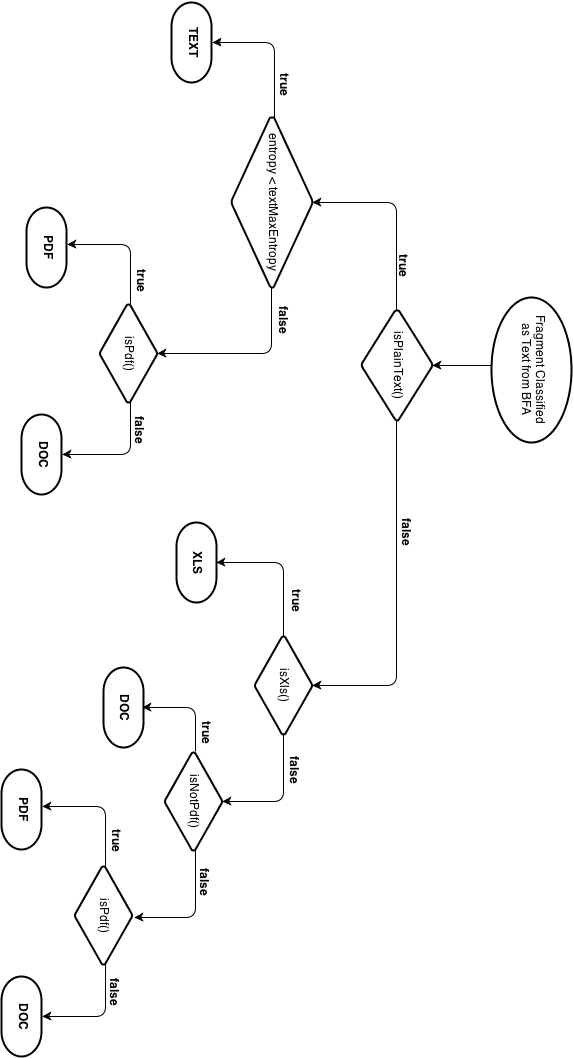
\includegraphics[scale=0.65]{./Figures/flowchart}
   \caption{Algorithm as Decision Tree\label{flowchart}}
\end{figure}

